\section{Results}
\label{sec:results}

All figures in this section are exact expectations over each profile's support. \Cref{fig:heat} gives each arm's worst safety failure rate over each family's profiles; \cref{tab:adv} gives the adversarial profile, which admits every fault the family models. \Cref{app:results} lists all 180 family--profile--arm rows.

\begin{figure}[t]
\centering
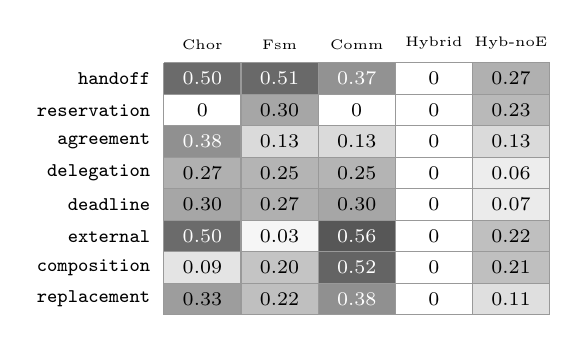
\begin{tikzpicture}[font=\scriptsize]
\node[anchor=south, font=\tiny] at (0.49,0.05) {\arm{Chor}};
\node[anchor=south, font=\tiny] at (1.47,0.05) {\arm{Fsm}};
\node[anchor=south, font=\tiny] at (2.45,0.05) {\arm{Comm}};
\node[anchor=south, font=\tiny] at (3.4299999999999997,0.05) {\arm{Hybrid}};
\node[anchor=south, font=\tiny] at (4.41,0.05) {\arm{Hyb-noE}};
\node[anchor=east] at (-0.05,-0.2) {\texttt{handoff}};
\fill[black!58.099999999999994] (0,-0.4) rectangle (0.98,0.0);
\node[text=white] at (0.49,-0.2) {0.50};
\fill[black!58.8] (0.98,-0.4) rectangle (1.96,0.0);
\node[text=white] at (1.47,-0.2) {0.51};
\fill[black!42.699999999999996] (1.96,-0.4) rectangle (2.94,0.0);
\node[text=white] at (2.45,-0.2) {0.37};
\fill[black!0] (2.94,-0.4) rectangle (3.92,0.0);
\node[text=black] at (3.4299999999999997,-0.2) {0};
\fill[black!30.799999999999997] (3.92,-0.4) rectangle (4.9,0.0);
\node[text=black] at (4.41,-0.2) {0.27};
\node[anchor=east] at (-0.05,-0.6000000000000001) {\texttt{reservation}};
\fill[black!0] (0,-0.8) rectangle (0.98,-0.4);
\node[text=black] at (0.49,-0.6000000000000001) {0};
\fill[black!35.0] (0.98,-0.8) rectangle (1.96,-0.4);
\node[text=black] at (1.47,-0.6000000000000001) {0.30};
\fill[black!0] (1.96,-0.8) rectangle (2.94,-0.4);
\node[text=black] at (2.45,-0.6000000000000001) {0};
\fill[black!0] (2.94,-0.8) rectangle (3.92,-0.4);
\node[text=black] at (3.4299999999999997,-0.6000000000000001) {0};
\fill[black!27.299999999999997] (3.92,-0.8) rectangle (4.9,-0.4);
\node[text=black] at (4.41,-0.6000000000000001) {0.23};
\node[anchor=east] at (-0.05,-1.0000000000000002) {\texttt{agreement}};
\fill[black!43.4] (0,-1.2000000000000002) rectangle (0.98,-0.8000000000000002);
\node[text=white] at (0.49,-1.0000000000000002) {0.38};
\fill[black!14.7] (0.98,-1.2000000000000002) rectangle (1.96,-0.8000000000000002);
\node[text=black] at (1.47,-1.0000000000000002) {0.13};
\fill[black!14.7] (1.96,-1.2000000000000002) rectangle (2.94,-0.8000000000000002);
\node[text=black] at (2.45,-1.0000000000000002) {0.13};
\fill[black!0] (2.94,-1.2000000000000002) rectangle (3.92,-0.8000000000000002);
\node[text=black] at (3.4299999999999997,-1.0000000000000002) {0};
\fill[black!14.7] (3.92,-1.2000000000000002) rectangle (4.9,-0.8000000000000002);
\node[text=black] at (4.41,-1.0000000000000002) {0.13};
\node[anchor=east] at (-0.05,-1.4000000000000001) {\texttt{delegation}};
\fill[black!30.799999999999997] (0,-1.6) rectangle (0.98,-1.2000000000000002);
\node[text=black] at (0.49,-1.4000000000000001) {0.27};
\fill[black!29.4] (0.98,-1.6) rectangle (1.96,-1.2000000000000002);
\node[text=black] at (1.47,-1.4000000000000001) {0.25};
\fill[black!29.4] (1.96,-1.6) rectangle (2.94,-1.2000000000000002);
\node[text=black] at (2.45,-1.4000000000000001) {0.25};
\fill[black!0] (2.94,-1.6) rectangle (3.92,-1.2000000000000002);
\node[text=black] at (3.4299999999999997,-1.4000000000000001) {0};
\fill[black!7.0] (3.92,-1.6) rectangle (4.9,-1.2000000000000002);
\node[text=black] at (4.41,-1.4000000000000001) {0.06};
\node[anchor=east] at (-0.05,-1.8) {\texttt{deadline}};
\fill[black!35.0] (0,-2.0) rectangle (0.98,-1.6);
\node[text=black] at (0.49,-1.8) {0.30};
\fill[black!30.799999999999997] (0.98,-2.0) rectangle (1.96,-1.6);
\node[text=black] at (1.47,-1.8) {0.27};
\fill[black!35.0] (1.96,-2.0) rectangle (2.94,-1.6);
\node[text=black] at (2.45,-1.8) {0.30};
\fill[black!0] (2.94,-2.0) rectangle (3.92,-1.6);
\node[text=black] at (3.4299999999999997,-1.8) {0};
\fill[black!7.699999999999999] (3.92,-2.0) rectangle (4.9,-1.6);
\node[text=black] at (4.41,-1.8) {0.07};
\node[anchor=east] at (-0.05,-2.2) {\texttt{external}};
\fill[black!58.099999999999994] (0,-2.4000000000000004) rectangle (0.98,-2.0000000000000004);
\node[text=white] at (0.49,-2.2) {0.50};
\fill[black!3.5] (0.98,-2.4000000000000004) rectangle (1.96,-2.0000000000000004);
\node[text=black] at (1.47,-2.2) {0.03};
\fill[black!65.8] (1.96,-2.4000000000000004) rectangle (2.94,-2.0000000000000004);
\node[text=white] at (2.45,-2.2) {0.56};
\fill[black!0] (2.94,-2.4000000000000004) rectangle (3.92,-2.0000000000000004);
\node[text=black] at (3.4299999999999997,-2.2) {0};
\fill[black!25.2] (3.92,-2.4000000000000004) rectangle (4.9,-2.0000000000000004);
\node[text=black] at (4.41,-2.2) {0.22};
\node[anchor=east] at (-0.05,-2.6) {\texttt{composition}};
\fill[black!10.5] (0,-2.8000000000000003) rectangle (0.98,-2.4000000000000004);
\node[text=black] at (0.49,-2.6) {0.09};
\fill[black!23.099999999999998] (0.98,-2.8000000000000003) rectangle (1.96,-2.4000000000000004);
\node[text=black] at (1.47,-2.6) {0.20};
\fill[black!60.9] (1.96,-2.8000000000000003) rectangle (2.94,-2.4000000000000004);
\node[text=white] at (2.45,-2.6) {0.52};
\fill[black!0] (2.94,-2.8000000000000003) rectangle (3.92,-2.4000000000000004);
\node[text=black] at (3.4299999999999997,-2.6) {0};
\fill[black!25.2] (3.92,-2.8000000000000003) rectangle (4.9,-2.4000000000000004);
\node[text=black] at (4.41,-2.6) {0.21};
\node[anchor=east] at (-0.05,-3.0) {\texttt{replacement}};
\fill[black!38.5] (0,-3.2) rectangle (0.98,-2.8000000000000003);
\node[text=black] at (0.49,-3.0) {0.33};
\fill[black!25.2] (0.98,-3.2) rectangle (1.96,-2.8000000000000003);
\node[text=black] at (1.47,-3.0) {0.22};
\fill[black!43.4] (1.96,-3.2) rectangle (2.94,-2.8000000000000003);
\node[text=white] at (2.45,-3.0) {0.38};
\fill[black!0] (2.94,-3.2) rectangle (3.92,-2.8000000000000003);
\node[text=black] at (3.4299999999999997,-3.0) {0};
\fill[black!12.6] (3.92,-3.2) rectangle (4.9,-2.8000000000000003);
\node[text=black] at (4.41,-3.0) {0.11};
\draw[black!40] (0,-3.2) grid[xstep=0.98,ystep=0.4] (4.9,0);
\end{tikzpicture}

\caption{Worst-profile safety failure rate: for each family and arm, the largest SFR over the family's profiles. Darker is less safe. Only \arm{Hybrid}'s column is zero throughout.}
\label{fig:heat}
\end{figure}

\begin{table}[t]
\centering
\caption{Adversarial profile: safety failure rate per arm; for \arm{Hybrid}, SFR / coverage.}
\label{tab:adv}
\small
\setlength{\tabcolsep}{4pt}
\begin{tabular}{@{}lccccc@{}}
\toprule
Family & \arm{Chor} & \arm{Fsm} & \arm{Comm} & \arm{Hybrid} & \arm{Hyb-noE} \\
\midrule
\tabinput{tables/adversarial}
\bottomrule
\end{tabular}
\end{table}

\subsection{Against the hypotheses}

The framework states six falsifiable hypotheses. DMBench as built tests four of them.

\paragraph{H1, responsibility} \emph{Explicit commitments reduce unowned-obligation time.} Supported in refined form. In \family{delegation} and \family{replacement}, the arm whose protocol releases the delegating party (\arm{Chor}) leaves responsibility unowned for a quarter of the required time (AGR 0.25 in both), while every arm that retains responsibility until the successor accepts has AGR 0. Retention, not the commitment vocabulary, carries the result: \arm{Fsm}'s guard retains responsibility as well as \arm{Comm}'s pending commitment does.

\paragraph{H2, safety, and H3, communication} \emph{Guarded state machines reduce unauthorized transitions; session-typed choreography reduces invalid traces.} Not tested. DMBench measures judgment about dependencies, not the admission of unauthorized transitions or ill-typed messages; both need fault classes (forged and malformed actions) that the families do not inject (\cref{sec:agenda}).

\paragraph{H4, observability} \emph{Explicit evidentiary semantics improve compliance classification.} Supported. \arm{Hybrid} makes no false claim in any family under any profile, and \arm{Hybrid-noE}, which differs only by E1--E3, is unsafe in every family. The independent arms reproduce both facts before adjudication.

\paragraph{H5, hybrid} \emph{Combining semantics improves multi-dimensional adequacy.} Supported as a trade-off, which is how the preregistered protocol states it, not as dominance. \arm{Hybrid} dominates on safety but not on coverage: in \family{external} its adversarial coverage is 0.48 where \arm{Comm} claims on every run and is false on 56\% of them.

\paragraph{H6, composition} \emph{Unchecked composition introduces compliance blind spots.} Supported. Under the coarse observation model the composition's stage dependency is determined in no world under any profile (\cref{tab:p2}).

\subsection{Further findings}

\paragraph{No single paradigm is adequate across the families} \arm{Chor} and \arm{Comm} make false claims in seven of the eight families and \arm{Fsm} in all eight; each is safe somewhere. \arm{Fsm} is safe in \family{handoff} under reliable delivery, but its own timeout fires on a dropped acceptance and it trusts stale state. \arm{Comm} is safe in \family{reservation} under every profile and unsafe in \family{external} under reliable delivery. \arm{Chor} is safe in \family{reservation} and unsafe in \family{agreement} under reliable delivery.

\paragraph{False completion follows the evidence model, not the paradigm} Wherever a participant reports its own performance, every arm that accepts the report produces false $\Ful$ claims: a premature start report in \family{handoff} gives FCR 0.467 for \arm{Chor}, \arm{Fsm} and \arm{Comm} alike under \texttt{evidence-contradiction}; a premature completion report in \family{external}, a subcontractor's premature self-report in \family{composition}, a skewed clock in \family{deadline} and a stale queued START in \family{replacement} do the same. \arm{Hybrid}'s FCR is zero throughout.

\paragraph{Operational and epistemic adequacy separate} In four families the arm's protocol features change truth (\cref{fig:opep}). In \family{reservation}, \arm{Chor} and \arm{Comm} regrant only on release: they never overcommit, so sharing always holds, but $h_2$ waits past its deadline whenever $h_1$ overruns, dies or its release is lost, a protocol-induced temporal violation that both arms judge correctly. \arm{Fsm}'s unfenced expiry regrant meets the deadline and lets an overrunning $h_1$ overlap $h_2$. The hybrid's fenced expiry gives both. An arm can be epistemically sound about a dependency its own conduct violates, and operationally adequate for a dependency it cannot observe.

\begin{figure}[t]
\centering
\footnotesize
\setlength{\tabcolsep}{3pt}
\renewcommand{\arraystretch}{1.25}
\begin{tabular}{@{}L{19mm} L{21mm} L{25mm} L{11mm}@{}}
\toprule
Arms, regrant rule & \texttt{sharing} & \texttt{temporal} & False claims \\
\midrule
\arm{Chor}, \arm{Comm}\newline\emph{on release} & holds in every world & violated when $h_1$ overruns, dies or its release is lost & none \\
\arm{Fsm}\newline\emph{on expiry} & violated when an overrunning $h_1$ overlaps $h_2$ & holds in every world & every profile \\
\arm{Hybrid}\newline\emph{expiry with fencing} & holds in every world & holds in every world & none \\
\bottomrule
\end{tabular}
\caption{Operational and epistemic adequacy separate in \family{reservation}. The regrant rule decides which dependency the protocol's own conduct violates. \arm{Chor} and \arm{Comm} judge their own violations correctly; \arm{Fsm} makes false claims under every profile. Only fenced expiry is operationally adequate for both dependencies.}
\label{fig:opep}
\end{figure}

\paragraph{Granularity is part of adequacy} In \family{external}, \arm{Comm} holds one conjunctive commitment for both parts of an order, so a pending internal part makes it claim the external part violated, which is false whenever the external executor completed it: SFR 0.25 under reliable delivery. The independent author's reading, one commitment per part with nothing the creditor holds able to discharge the external one, is false whenever the executor completes the part.

\paragraph{Timing faults break arms that judge by arrival or by a party's clock} In \family{deadline}, \arm{Chor} and \arm{Comm} judge by the completion report's arrival and are false under transit delay (SFR 0.30); \arm{Fsm} judges by the provider's stamp and is safe under delay but false under clock skew (0.27); the hybrid uses the trusted stamp. In \family{handoff}, a timely acceptance with a slow reply takes \arm{Chor}'s and \arm{Fsm}'s timeout branch (SFR 0.30 under \texttt{timing}).

\subsection{Family by family}

\paragraph{\family{handoff}} The family in which observation is hardest: under the adversarial profile the single-paradigm arms' observations determine at most 0.31 of outcomes. \arm{Fsm} is the least safe arm (SFR 0.51), because it reads stale state as current and its own timeout fires on dropped and slow acceptances; \arm{Comm} is safe under lossy delivery and timing variation but not under stale reads (0.37). The premature start report produces the paradigm-independent FCR of 0.467 described above.

\paragraph{\family{reservation}} Operational adequacy, not judgment, separates the arms (\cref{fig:opep}). \arm{Chor} and \arm{Comm} are safe under every profile, about outcomes their own conduct makes worse. The ablation, which drops the fencing tokens as well as E1--E3, is the only variant of the hybrid that loses observation.

\paragraph{\family{agreement}} Concurrent revocation is harmless to every arm whose binding waits for the seller's acknowledgement. \arm{Chor}'s binding on send, with no check of the seller's terms, is unsafe under every profile (SFR 0.25 to 0.38); \arm{Fsm} and \arm{Comm} fail only when a stale read is taken over an absent acknowledgement (0.13).

\paragraph{\family{delegation}} Releasing the delegator (\arm{Chor}) leaves a quarter of the required responsibility time unowned in every profile, and when a later START replaces the delegation in its session view it claims continuity that did not hold (FCR 0.40 under lossy delivery). The retaining arms have no gap; \arm{Fsm} and \arm{Comm} fail only on stale reads (0.25).

\paragraph{\family{deadline}} Every fault leaves a distinct trace, so every arm's observations determine every outcome; all failures are interpretive. Judging by arrival fails under transit delay and judging by the provider's clock fails under skew, as reported above.

\paragraph{\family{external}} The executor is outside every protocol, so only an interface that carries its receipt can determine the external part. \arm{Fsm} abstains on it everywhere and is nearly safe (0.03); \arm{Chor} and \arm{Comm} read the provider's completion report as covering the external part and are false on half the runs under premature reports. The hybrid's coverage (0.48) is the lowest of any arm because E1 forbids it to accept the provider's own record of its own part.

\paragraph{\family{composition}} Under the coarse model the single-paradigm arms can determine only the delivery dependency (0.38 of claims). \arm{Comm}'s creditor rule makes it claim the stage violated on every run without evidence, and it is false on half of them; \arm{Fsm} infers the stage from a closed case and is false when the stage was late.

\paragraph{\family{replacement}} The stale queued START passes for the debtor's start when $V$ has resumed the role, and fools \arm{Comm} and the ablation; \arm{Chor}, which credits only the current session's party, is not fooled, but its timeouts on dropped notices make it as unsafe as \arm{Comm} under stale reads (0.33). Releasing the withdrawing party leaves a quarter of the required time unowned, as in \family{delegation}.

\subsection{The ceiling on sound judgment}

\Cref{tab:ceiling} sets \arm{Hybrid}'s supported share against the ceiling of \cref{thm:ceiling}, its determinable share. In \family{agreement}, \family{handoff}, \family{delegation} and \family{replacement} the hybrid is within 0.07 of the ceiling. Where it is further away the cause is one of two kinds. In \family{reservation} and \family{deadline} the gap is guarantees by construction or inferences from the model's narrowness that the hybrid declines to make without run evidence (\cref{sec:limitations}). In \family{external} and \family{composition} it is the evidence rules themselves: E1 forbids the hybrid to accept $V$'s own record of $V$'s performance, and the composition's case record carries no watermark for E2 to use.

\begin{table}[t]
\centering
\caption{Ceiling on sound judgment, adversarial profile. Det.: determinable share for \arm{Hybrid} (the ceiling); Sup.: its supported share; Miss: its abstained-miss share. Last three columns: determinable share for the single-paradigm arms.}
\label{tab:ceiling}
\small
\setlength{\tabcolsep}{3.5pt}
\begin{tabular}{@{}lcccccc@{}}
\toprule
& \multicolumn{3}{c}{\arm{Hybrid}} & \multicolumn{3}{c}{Determinable} \\
\cmidrule(lr){2-4}\cmidrule(l){5-7}
Family & Det. & Sup. & Miss & \arm{Chor} & \arm{Fsm} & \arm{Comm} \\
\midrule
\tabinput{tables/ceiling}
\bottomrule
\end{tabular}
\end{table}

The single-paradigm columns show the other half of \cref{cor:interface}. In \family{handoff} the single-paradigm arms' observations determine at most 0.31 of the outcomes under the adversarial profile, so no judge over those observations, however careful, could be sound with coverage above 0.31; the hybrid's interface raises the ceiling to 0.56.

\subsection{Propositions}

\paragraph{P1} \Cref{tab:p1} counts observation classes containing worlds with different truth. Witnesses exist in every family except \family{deadline}, where every fault leaves a distinct trace and the difficulty is interpretation, not observation.

\begin{table}[t]
\centering
\caption{P1 witnesses: ambiguous observation classes, summed over profiles.}
\label{tab:p1}
\small
\setlength{\tabcolsep}{4pt}
\begin{tabular}{@{}lccccc@{}}
\toprule
Family & \arm{Chor} & \arm{Fsm} & \arm{Comm} & \arm{Hybrid} & \arm{Hyb-noE} \\
\midrule
\tabinput{tables/p1}
\bottomrule
\end{tabular}
\end{table}

\paragraph{P2} \Cref{tab:p2} and \cref{fig:p2} run the hybrid's protocol in \family{composition} under three observation models of $V$'s case. Under the coarse model the stage dependency is never determined; the staged model determines it fully only when $S$ reports honestly; an attestation of $S$'s start restores it.

\begin{figure}[t]
\centering
\begin{tikzpicture}[font=\scriptsize, >=Stealth,
  p/.style={draw, circle, minimum size=6mm, inner sep=0pt}]
\node[p] (S) at (0,0) {$S$};
\node[p] (V) at (2.4,0) {$V$};
\node[p] (H) at (4.6,0) {$H$};
\draw[->] (S) -- node[above, font=\tiny]{$\sigma$: self-report} (V);
\draw[->] (V) -- node[above, font=\tiny]{case view} (H);
\node[draw, rounded corners=2pt, inner sep=2pt] (A) at (2.4,-0.85) {attester};
\draw[->, densely dashed] (S) |- (A);
\draw[->, densely dashed] (A) -| node[pos=0.25, below]{start stamp} (H);
\begin{scope}[shift={(0.2,-1.9)}]
\foreach \i/\m/\r/\s in {0/coarse/0/0, 1/staged/1/0.25, 2/staged+attest/1/1}{
  \node[anchor=east] at (0.95,-\i*0.42-0.12) {\texttt{\m}};
  \fill[black!65] (1,-\i*0.42-0.2) rectangle ++(\r*2.4,0.16);
  \fill[black!25] (1,-\i*0.42-0.38) rectangle ++(\s*2.4,0.16);
}
\draw (1,0.05) -- (1,-1.3);
\draw (3.4,0.05) -- (3.4,-1.3) node[below]{1};
\node[below] at (1,-1.3) {0};
\fill[black!65] (3.7,-0.3) rectangle ++(0.25,0.12); \node[anchor=west] at (3.95,-0.24) {\texttt{reliable}};
\fill[black!25] (3.7,-0.62) rectangle ++(0.25,0.12); \node[anchor=west] at (3.95,-0.56) {\texttt{self-report}};
\end{scope}
\end{tikzpicture}
\caption{P2 in the composition family. $H$ observes $S$ only through $V$'s relay of $S$'s self-report $\sigma$, unless an attester stamps $S$'s start. Bars: determinable mass of $H$'s stage dependency under each observation model, with honest reporting (\texttt{reliable}) and with premature reports admitted (\texttt{self-report}).}
\label{fig:p2}
\end{figure}

\begin{table}[t]
\centering
\caption{P2: determinable mass of the composition's dependencies under three observation models of $V$'s case. Amb.: ambiguous observation classes.}
\label{tab:p2}
\footnotesize
\setlength{\tabcolsep}{3pt}
\begin{tabular}{@{}llccc@{}}
\toprule
Profile & Model & Amb. & \texttt{temporal} & \texttt{delivery} \\
\midrule
\tabinput{tables/p2}
\bottomrule
\end{tabular}
\end{table}

\paragraph{P3} \Cref{tab:p3} compares \arm{Hybrid} with each variant: world--dependency pairs where the variant makes a false claim the hybrid does not (safety lost) and where an outcome determined for the hybrid is not determined for the variant (observation lost). The ablation loses safety in every family and observation only in \family{reservation}, the one family where it also changes conduct.

\begin{table}[t]
\centering
\caption{P3: \arm{Hybrid} against each variant, summed over profiles; safety lost / observation lost.}
\label{tab:p3}
\small
\setlength{\tabcolsep}{4pt}
\begin{tabular}{@{}lcccc@{}}
\toprule
Family & \arm{Hyb-noE} & \arm{Chor} & \arm{Fsm} & \arm{Comm} \\
\midrule
\tabinput{tables/p3}
\bottomrule
\end{tabular}
\end{table}
